\pdfoutput=1
\documentclass[a4paper,pdflatex,ja=standard]{bxjsarticle}

% ---Setting about the geometry of the document----
% \usepackage{a4wide}
% \pagestyle{empty}

% ---Physics and Math Packages---
\usepackage{amssymb,amsfonts,amsthm,mathtools}
\usepackage{physics,braket,bm}

% ---underline---
\usepackage{ulem}

% --- sorround the texts or equations
% \usepackage{fancybox,ascmac}

% ---settings of theorem environment---
% \usepackage{amsthm}
% \theoremstyle{definition}

% ---settings of proof environment---
% \renewcommand{\proofname}{\uline{\textbf{証明}}}
% \renewcommand{\qedsymbol}{$\blacksquare$}

% ---Ignore the Warnings---
\usepackage{silence}
\WarningFilter{latexfont}{Some font shapes,Font shape}

% ---Insert the figure (If insert the `draft' at the option, the process becomes faster)---
\usepackage{graphicx}
% \usepackage{subcaption}

% ----Add a link to a text---
\usepackage{url}
\usepackage{xcolor,hyperref}
\hypersetup{colorlinks=true,citecolor=orange,linkcolor=blue,urlcolor=magenta}
\usepackage{bxcjkjatype}

% ---Tikz---
\usepackage{tikz,pgf,pgfplots,circuitikz}
\pgfplotsset{compat=1.15}
\usetikzlibrary{intersections,arrows.meta,angles,calc,3d,decorations.pathmorphing}

% ---Add the section number to the equation, figure, and table number---
\makeatletter
   \renewcommand{\theequation}{\thesubsection.\arabic{equation}}
   \@addtoreset{equation}{subsection}
   
   \renewcommand{\thefigure}{\thesection.\arabic{figure}}
   \@addtoreset{figure}{section}
   
   \renewcommand{\thetable}{\thesection.\arabic{table}}
   \@addtoreset{table}{section}
\makeatother

% ---enumerate---
\renewcommand{\labelenumi}{\arabic{enumi}.}
\renewcommand{\labelenumii}{(\roman{enumii})}
\renewcommand{\labelenumiii}{(\alph{enumiii})}

% ---Index---
% \usepackage{makeidx}
% \makeindex

% ---Fonts---
\renewcommand{\familydefault}{\sfdefault}

% ---Title---
\title{東京大学\ 平成25年\ 物理学専攻\ 院試\ 解答例}
\author{ミヤネ}
\date{最終更新:\today}

\newcommand{\prb}[2]{
  \phantomsection
  \addcontentsline{toc}{subsection}{問題 #1: #2}
  \subsection*{第#1問\phantom{#2}}
  \setcounter{subsection}{#1}
  \setcounter{equation}{0}
}

\begin{document}

\maketitle

\tableofcontents
\clearpage


\section{数学パート}

\prb{1}{線形代数・複素関数}

\begin{enumerate}
  
  \item 

  \begin{enumerate}

    \item
    
    左辺については,行列式の定義より
    \begin{equation}
      \Delta(\vec{z})
      =
      \sum_{\sigma}
      \mathrm{sgn}(\sigma)
      x_{1\sigma(1)}
      x_{2\sigma(2)}
      x_{3\sigma(3)}
      x_{4\sigma(4)}
    \end{equation}
    です.ここで,$x_{1\sigma(1)}$は0次,$x_{2\sigma(2)}$は1次,$x_{3\sigma(3)}$は2次,$x_{4\sigma(4)}$は3次なので,$\Delta(\vec{z})$は6次の同次多項式です.一方で,右辺が6次の同次多項式なのは明らか.


    \item 

    行列式は,列が一致するときは基本変形で1列を0にすることができるので,行列式の定義で$x_{1\sigma(1)}=0$となり,$\Delta(\vec{z})=0$.


    \item 

    比例定数を$k$としましょう.つまり
    \begin{equation}
      \Delta(\vec{z})
      =
      k(z_1-z_2)(z_1-z_3)(z_1-z_4)(z_2-z_3)(z_2-z_4)(z_3-z_4)
    \end{equation}
    とします.両辺の$z_2z_3^2z_4^3$の項を比較すると$k=1$が示されるので,式(1)が成立します。


  \end{enumerate}


  \item 

  \begin{enumerate}

    \item 

    \begin{equation}
      \frac{1}{g(z)}\dv{g(z)}{z}
      =
      \dv{\lambda(z)}{z}
      ,\ 
      \frac{1}{g(z)}\dv[2]{g(z)}{z}      
      =
      \dv[2]{\lambda(z)}{z}
      +
      \left( \dv{\lambda(z)}{z} \right)^2
      .
    \end{equation}


    \item 

    前問の結果を用いて$f(z)$を計算すると
    \begin{align}
      f(z)
      &=
      \pdv[2]{}{z_1}\log \Delta(\vec{z})
      +
      \left(  
        \pdv{}{z_1}\log \Delta(\vec{z})
      \right)
      \nonumber
      \\
      &=
      -
      \frac{1}{(z_1-z_2)^2}
      -
      \frac{1}{(z_1-z_3)^2}
      -
      \frac{1}{(z_1-z_4)^2}
      +
      \left(  
        \frac{1}{z_1-z_2}
        +
        \frac{1}{z_1-z_3}
        +
        \frac{1}{z_1-z_4}
      \right)^2
      \nonumber
      \\
      &=
      \frac{2}{(z_1-z_2)(z_1-z_3)}
      +
      \frac{2}{(z_1-z_3)(z_1-z_4)}
      +
      \frac{2}{(z_1-z_4)(z_1-z_2)}
      \nonumber
      \\
      &=
      \left( \frac{1}{z_1-z_2}-\frac{1}{z_1-z_3} \right)\frac{2}{z_2-z_3}
      +
      \left( \frac{1}{z_1-z_3}-\frac{1}{z_1-z_4} \right)\frac{2}{z_3-z_4}
      \nonumber
      \\
      &\hspace{7cm}
      +
      \left( \frac{1}{z_1-z_4}-\frac{1}{z_1-z_2} \right)\frac{2}{z_4-z_2}
    \end{align}
    となるので,極は1次のみです.


    \item 

    例えば,$1/(z_1-z_2)$の項は
    \begin{equation}
      \oint\frac{\dd z_1}{2\pi i}
      \frac{z_1}{z_1-z_2}
      =
      z_2
    \end{equation}
    となることに注意すれば
    \begin{equation}
      \oint\frac{\dd z_1}{2\pi i}
      z_1f(z)
      =
      6
      .
    \end{equation}

  \end{enumerate}


\end{enumerate}



\clearpage

\prb{2}{微積分}

総和の記号$\sum$は省きます.

\begin{enumerate}

  \item 

  \begin{equation}
    \begin{pmatrix}
      \dfrac{\partial}{\partial x_1} \\
      \dfrac{\partial}{\partial x_2}
    \end{pmatrix}
    =
    C^{T}
    \begin{pmatrix}
      \dfrac{\partial}{\partial \xi_1} \\
      \dfrac{\partial}{\partial \xi_2}
    \end{pmatrix}
    .
  \end{equation}


  \item 

  $A\equiv(a_{ij})$とおくと,2階微分の項は
  \begin{equation}
    a_{ij}\pdv{}{x_i}{x_j}
    =
    \begin{pmatrix}
      \pdv{}{x_1} & \pdv{}{x_2}
    \end{pmatrix}
    A
    \begin{pmatrix}      
      \pdv{}{x_1} \\
      \pdv{}{x_2}
    \end{pmatrix}
    =
    \begin{pmatrix}
      \pdv{}{\xi_1} & \pdv{}{\xi_2}
    \end{pmatrix}
    CAC^{T}
    \begin{pmatrix}      
      \pdv{}{\xi_1} \\
      \pdv{}{\xi_2}
    \end{pmatrix}
  \end{equation}
  と変換できます.行列$A$の固有値を$\lambda_1,\lambda_2$とおき,$v_1,v_2$をそれに対応する規格化された固有ベクトルとしましょう.$A$は対称行列なので,直交行列を用いて対角化することができます.その対角化行列を$P$とおきましょう.$C=P^{T}$ととれば
  \begin{equation}
    \begin{pmatrix}
      \lambda_1 & 0 \\
      0 & \lambda_2
    \end{pmatrix}
    =
    CAC^{T}
  \end{equation}
  となります.ここで,$C^T=C^{-1}$より,$D=\det A=\lambda_1\lambda_2$に注意してださい.

  \begin{itemize}

    \item 
    
    \uline{$D>0$のとき}

    $C$を
    \begin{equation}
      C^T
      =
      \begin{pmatrix}
        \frac{1}{\sqrt{|\lambda_1|}}v_1
        &
        \frac{1}{\sqrt{|\lambda_2|}}v_2
      \end{pmatrix}
    \end{equation}
    を満たすようにとると,
    \begin{equation}
      CAC^T
      =
      \pm 
      \begin{pmatrix}
        1 & 0 \\
        0 & 1
      \end{pmatrix}
    \end{equation}
    とすることができます.よって,このとき
    \begin{equation}
      a_{ij}\pdv{}{x_i}{x_j}
      =
      \pm
      \left(  
        \pdv[2]{}{\xi_1}
        +
        \pdv[2]{}{\xi_2}
      \right)
    \end{equation}
    となります\footnote{
      マイナスになるかどうかは,$\lambda_1$と$\lambda_2$の符号によります.$\lambda_1\lambda_2>0$より,$\lambda_1,\lambda_2$の符号は同じなので,$\pm$はカッコの外側にあることに気をつけてください.
    }.


    \item 

    \uline{$D=0$のとき}

    $\lambda_1\lambda_2=0$なので,$\lambda_1=0$とおきます.すると,$D>0$の場合と同じように$C$をとれば,同じ議論から
    \begin{equation}
      a_{ij}\pdv{}{x_i}{x_j}
      =
      \pm
      \pdv[2]{}{\xi_2}
    \end{equation}
    となります.


    \item 

    \uline{$D<0$のとき}

    $\lambda_1>0, \lambda_2<0$ととります.すると,また同じ議論から
    \begin{equation}
      a_{ij}\pdv{}{x_i}{x_j}
      =
      \pdv[2]{}{\xi_1}
      -
      \pdv[2]{}{\xi_2}
    \end{equation}
    となります.


  \end{itemize}


  \item 

  同様に$b\equiv(b_i)$とおき,$b'\equiv C^{T}b$とすれば,1階微分の項は
  \begin{equation}
    b_i\pdv{}{x_i}
    =
    b'_1\pdv{}{\xi_1}
    +
    b'_2\pdv{}{\xi_2}
  \end{equation}
  と書けます.

  \begin{itemize}

    \item 

    \uline{$D>0$のとき}

    前問の結果と合わせれば,偏微分方程式$\mathcal{L}\psi=E\psi$が
    \begin{equation}
      \left[  
        \pdv[2]{}{\xi_1}
        +
        \pdv[2]{}{\xi_2}
        +        
        b'_1\pdv{}{\xi_1}
        +
        b'_2\pdv{}{\xi_2}
      \right]
      e^{\lambda_1\xi_1+\lambda_2\xi_2}\phi
      =
      E
      e^{\lambda_1\xi_1+\lambda_2\xi_2}\phi
    \end{equation}
    となるように$C$をとることができます.微分の部分を計算すると
    \begin{align}     
      &\hspace{-2cm}
      \left[  
        \uwave{
          \pdv[2]{}{\xi_1}
          +
          \pdv[2]{}{\xi_2}
        }
        +        
        \uline{
          b'_1\pdv{}{\xi_1}
          +
          b'_2\pdv{}{\xi_2}
        }
      \right]
      e^{\lambda_1\xi_1+\lambda_2\xi_2}
      \phi
      \nonumber
      \\
      &=
      e^{\lambda_1\xi_1+\lambda_2\xi_2}
      \left[  
        \uwave{
          \lambda_1^2+\lambda_2^2
          +
          2\lambda_1\pdv{}{\xi_1}+2\lambda_2\pdv{}{\xi_2}
          +
          \pdv[2]{}{\xi_1}
          +
          \pdv[2]{}{\xi_2}
        }
      \right.
      \nonumber
      \\
      &\hspace{4.2cm}
      \left.
        +
        \uline{
          b'_1\left( \lambda_1+\pdv{}{\xi_1} \right)
          +
          b'_2\left( \lambda_2+\pdv{}{\xi_2} \right)
        }
      \right]
      \phi
      \label{diff_term}
    \end{align}
    となりますが,$\lambda_1,\lambda_2$を1階微分が消えるようにとり\footnote{
      $\lambda_1=-b'_1/2,\lambda_2=-b'_2/2$ととればよいでしょう.
    },定数項を移項してそれらをまとめて$F$とおけば式(2)になります.


    \item 

    \uline{$D=0$のとき}

    微分の部分\eqref{diff_term}は,この場合は
    \begin{equation}
      \lambda_2^2
      +
      2\lambda_2\pdv{}{\xi_2}
      +
      \pdv[2]{}{\xi_2}
      +
      b'_1\left( \lambda_1+\pdv{}{\xi_1} \right)
      +
      b'_2\left( \lambda_2+\pdv{}{\xi_2} \right)
    \end{equation}
    となるので,$\xi_2$の1階微分は$\lambda_2$の取り方で消えます.$\xi_1$の1階微分は消えないので,式(3)のようになります.


    \item 

    \uline{$D<0$のとき}

    $D>0$のときと同じ.


  \end{itemize}


  \item 

  \begin{enumerate}

    \item 

    代入するだけ.


    \item 

    $f(y)=1/2\pi$なので\footnote{
      ただし,
      $$
        \delta(\xi_2)
        =
        \frac{1}{2\pi}
        \int_{-\infty}^{\infty} e^{-iy\xi_2}
        \dd y 
      $$
      としました.
    },
    \begin{equation}
      \phi(\xi_1,\xi_2)
      =
      \frac{1}{2\sqrt{\pi\xi_1}}
      e^{-\frac{\xi_2^2}{\xi_1}}
      .
    \end{equation}

  \end{enumerate}

  \item 

  \begin{equation}
    \left(  
      \pdv[2]{}{\xi_1}
      -
      \pdv[2]{}{\xi_2}    
    \right)
    \phi
    =
    G_1^{\prime\prime}
    +
    G_2^{\prime\prime}
    -
    \left(  
      G_1^{\prime\prime}
      +
      G_2^{\prime\prime}
    \right)
    =
    0
    .
  \end{equation}


\end{enumerate}



\clearpage

\section{物理パート}

\prb{1}{量子力学}

ハット$\hat{\quad}$は省略します.

\begin{enumerate}

  \item 

  ア:$\sqrt{\dfrac{m\omega}{2\hbar}}x-\dfrac{i}{\sqrt{2m\hbar\omega}}p$.\\
  イ:$1$.\\
  ウ:$x=\sqrt{\dfrac{\hbar}{2m\omega}}(a+a^{\dag}) $.\\
  エ:$p=-i\sqrt{\dfrac{m\hbar\omega}{2}}(a-a^{\dag})$.\\
  オ:$\hbar\omega\left( a^{\dag}a+\dfrac{1}{2} \right)$.\\
  カ:$E_0=\dfrac{\hbar\omega}{2} $.\\
  キ:$\dfrac{1}{\sqrt{n+1}} $.\\
  ク:$E_n=\hbar\omega\left( n+\dfrac{1}{2} \right) $.


  \item 

  Schrödinger方程式
  \begin{equation}
    i\hbar\ket{\psi(t)}
    =
    H\ket{\psi(t)}
  \end{equation}
  に式(3)を代入すると
  \begin{equation}
    i\hbar\dv{c_n(t)}{t}
    =
    \hbar\omega\left(n+\frac{1}{2}\right)c_n(t)
  \end{equation}
  となるので,これを解けば
  \begin{equation}
    c_n(t)
    =
    c_n(0)
    \exp\left[ -i\omega\left( n+\frac{1}{2} \right)t \right]
    \label{ans2_2}
  \end{equation}
  となります.


  \item 

  $a\ket{\phi_n}=c_n\ket{\phi_{n-1}}$とすると$|c_n|^2=\mel*{\phi_n}{a^{\dag}a}{\phi_n}=n$なので,$c_n=\sqrt{n}$です.よって,
  \begin{align}
    (\Delta x)^2
    &=
    \mel*{\phi_n}{x^2}{\phi}
    -
    (\mel*{\phi_n}{x}{\phi_n})^2
    \nonumber
    \\
    &=
    \frac{\hbar}{2m\omega}
    (\mel*{\phi_n}{aa^{\dag}}{\phi_n}+\mel*{\phi_n}{a^{\dag}a}{\phi_n})
    \nonumber
    \\
    &=
    \frac{\hbar}{2m\omega}(2n+1)
  \end{align}
  です.$p$についても
  \begin{align}
    (\Delta p)^2
    &=
    \mel*{\phi_n}{p^2}{\phi_n}
    -
    (\mel*{\phi_n}{p}{\phi_n})^2
    \nonumber
    \\
    &=    
    -\frac{m\hbar\omega}{2}
    (\mel*{\phi_n}{aa^{\dag}}{\phi_n}+\mel*{\phi_n}{a^{\dag}a}{\phi_n})
    \nonumber
    \\
    &=
    \frac{m\hbar\omega}{2}(2n+1)
  \end{align}
  となるので,
  \begin{equation}
    \Delta x\cdot\Delta p
    =
    \hbar
    \left( n+\frac{1}{2} \right)
  \end{equation}
  です.


  \item

  $a$を$\ket{\alpha}$に作用させると,
  \begin{equation}
    a\ket{\alpha}
    =
    e^{-|\alpha|^2/2}\sum_{n=0}^{\infty}\frac{\alpha^n}{\sqrt{n!}}\cdot\sqrt{n}\ket{\phi_{n-1}}
    =
    \alpha\ket{\phi_n}
  \end{equation}
  となるので,確かに固有状態です.共役をとると$\bra{\phi_n}a^{\dag}=\alpha^{\ast}\bra{n}$.また,$\mel*{\alpha}{\alpha}=1$なので\footnote{
    ちゃんと計算すると
    \begin{align*}
      \ev*{\alpha|\alpha}
      &=
      e^{-r^2}
      \sum_{m=0}^{\infty}\sum_{n=0}^{\infty}
      \frac{(re^{-i\theta})^m(re^{i\theta})^n}{\sqrt{m!n!}}\ev*{\phi_m|\phi_n}
      \\
      &=
      e^{-r^2}
      \cdot
      \underbrace{
        \sum_{n=0}^{\infty}\frac{r^{2n}}{n!}
      }_{=e^{r^2}}
      =
      1
    \end{align*}
    となります.
  },
  \begin{equation}
    \mel*{\alpha}{x}{\alpha}
    =
    \sqrt{\frac{\hbar}{2m\omega}}(\alpha+\alpha^{\ast})
    =
    \sqrt{\frac{2\hbar}{m\omega}}r\cos\theta
  \end{equation}
  であり,
  \begin{equation}
    \ev*{\alpha|p|\alpha}
    =
    -i\sqrt{\frac{m\hbar\omega}{2}}(\alpha-\alpha^{\ast})
    =
    \sqrt{2m\hbar\omega}r\sin\theta
  \end{equation}
  です.


  \item 

  初期条件は
  \begin{equation}
    \ket{\psi(0)}
    =
    \sum_{n=0}^{\infty}
    e^{-r_0^2}\frac{r^n_0}{\sqrt{n!}}
    \ket{\phi_n}
  \end{equation}
  なので,設問2の答え\eqref{ans2_2}に
  \begin{equation}
    c_n(0)
    =
    e^{-r_0^2/2}\frac{r^n_0}{\sqrt{n!}}
  \end{equation}
  を代入して
  \begin{equation}
    c_n(t)
    =
    \frac{r^n_0}{\sqrt{n!}}
    \exp\left[ -\frac{r^2_0}{2}-i\omega\left( n+\frac{1}{2} \right)t \right]
  \end{equation}
  となるので
  \begin{equation}
    \ket{\psi(t)}
    =
    \sum_{n=0}^{\infty}
    \frac{r^n_0}{\sqrt{n!}}
    \exp\left[ -\frac{r^2_0}{2}-i\omega\left( n+\frac{1}{2} \right)t \right]
    \ket{\phi_n}
  \end{equation}
  です.また,$\ket{\psi(t)}$に$a$を作用させてみると
  \begin{equation}
    a\ket{\psi(t)}
    =
    r_0e^{-i\omega t}\ket{\psi(t)}
  \end{equation}
  となっているので
  \begin{equation}
    \mel*{\psi(t)}{X}{\psi(t)}
    =
    \frac{1}{\sqrt{2}}
    \mel*{\psi(t)}{(a+a^{\dag})}{\psi(t)}   
    =
    \sqrt{2}r_0\cos\omega t 
  \end{equation}
  です\footnote{
    $\ev*{\psi(t)|\psi(t)}=1$です.規格化は条件は,時間発展させても変化しないので.
  }.同様にして
  \begin{equation}
    \mel*{\psi(t)}{P}{\psi(t)}
    =
    \sqrt{2}r_0\cos\omega t 
  \end{equation}
  となるので,$\ev*{X}^2+\ev*{P}^2=2r_0^2$となり,円運動.


\end{enumerate}



\clearpage

\prb{2}{統計力学}

\begin{enumerate}

  \item 

  粒子の平均数は
  \begin{equation}
    \ev*{N}
    =
    \frac{1}{\beta}\pdv{}{\mu}\log\Theta
    =
    \sum_{i}
    \frac{1}{\beta}\pdv{}{\mu}\log\Theta_i
    =
    \sum_{i}
    \frac{1}{e^{\beta(\varepsilon_i-\mu)}-1}
  \end{equation}
  となるので,確かに$f(\varepsilon_i)$は第$i$状態にある粒子数の平均.


  \item 

  ボゾンだけ
  \quad
  基底状態
  \quad
  縮退し
  \quad
  極低温の
  \quad
  臨界温度
  \quad
  (31字)


  \item 

  臨界温度は
  \begin{equation}
    \rho
    =
    A(k_BT_c)^{3/2}
    \underbrace{
      \int_{0}^{\infty}\frac{\sqrt{x}}{e^x-1}\dd x
    }_{=I_1}
  \end{equation}
  となるので,
  \begin{equation}
    l
    \sim  
    \left(  
      \frac{I_1}{A(k_BT_c)^{3/2}}
    \right)^{1/3}
    \sim
    \left( \frac{\hbar^2}{mk_BT_c} \right)^{1/2}
    \sim
    \lambda_T
  \end{equation}
  です.


  \item

  エネルギーも
  \begin{equation}
    E
    =
    A\int_{0}^{\infty}
    \frac{\varepsilon^{3/2}}{e^{\beta\varepsilon}-1}
    \dd \varepsilon
    =
    A(k_BT)^{5/2}
    \underbrace{
      \int
      \frac{\varepsilon^{3/2}}{e^{\beta\varepsilon}-1}
      \dd \varepsilon
    }_{=I_2}
  \end{equation}
  となるので,$\gamma=3/2$です.

  \item 

  ギブスの関係式$\dd U=T\dd S$より
  \begin{equation}
    S
    =
    \int
    \frac{C_V(T)}{T}
    \dd T
  \end{equation}
  なので,$\nu=3/2$.


  \item 

  状態密度に関しては,問題文の式(3)が成り立っているとします.すると, 基底状態にいない粒子数$\tilde{\rho}$は
  \begin{align}
    \tilde{\rho}
    &=
    A\int_{\varepsilon_{\mathrm{z}}}^{\infty}
    \frac{(\varepsilon-\varepsilon_{\mathrm{z}})^{1/2}}{e^{\varepsilon}-1}
    \dd \varepsilon
    +
    A\int_{0}^{\infty}
    \frac{\varepsilon^{1/2}}{e^{\varepsilon}-1}
    \dd \varepsilon
    +
    A\int_{-\varepsilon_{\mathrm{z}}}^{\infty}
    \frac{(\varepsilon+\varepsilon_{\mathrm{z}})^{1/2}}{e^{\varepsilon}-1}
    \dd \varepsilon
    \nonumber
    \\
    &=
    A\int_{0}^{\infty}
    \frac{{\varepsilon^{\prime}}^{1/2}}{e^{\varepsilon^{\prime}+\varepsilon_{\mathrm{z}}}-1}
    \dd \varepsilon^{\prime}
    +
    \underbrace{A\int_{0}^{\infty}
    \frac{\varepsilon^{1/2}}{e^{\varepsilon}-1}
    \dd \varepsilon}_{\propto T^{3/2}}
    +
    A\int_{0}^{\infty}
    \frac{{\varepsilon^{\prime}}^{1/2}}{e^{\varepsilon^{\prime}-\varepsilon_{\mathrm{z}}}-1}
    \dd \varepsilon^{\prime}
  \end{align}
  となりますが,$\varepsilon^{\prime}$を上昇させていくと第1項と第3項の寄与は減少します\footnote{
    もう少し説明すると,第1項の減少度合いが,第3項の上昇度合いよりも強いので,第1,3項のトータルで減少していきます.このことに関しては,
    $$
      f(\varepsilon_z)
      =
      \frac{1}{e^{\varepsilon'+\varepsilon_{\mathrm{z}}}-1}
      +
      \frac{1}{e^{\varepsilon'-\varepsilon_{\mathrm{z}}}-1}
    $$
    という関数を評価してみると良いかもしれません.(ちょっとチェックしてみましたが,傾向は見えてました.)
  }.今,断熱変化を考えているため,BECは起き続けて$\tilde{\rho}=\mathrm{const.}$です.以上より,第2項の寄与が大きくなるため,$T$は上昇すると考えられます.


\end{enumerate}



\clearpage

\prb{3}{電磁気学}

\begin{enumerate}

  \item 

  \begin{equation}
    m\dv[2]{\bm{r}}{t}
    +
    q\dv{\bm{A}}{t}
    =
    q
    \left\{  
      \nabla
      \left(  
        \dv{\bm{r}}{t}
        \cdot
        \bm{A}
      \right)
      -
      \bm{\nabla}\varphi
    \right\}
    .
    \label{eom}
  \end{equation}


  \item 

  \eqref{eom}を整理すると
  \begin{equation}
    m\dv[2]{\bm{r}}{t}
    =
    q
    \left\{  
      \bm{\nabla}
      \left(  
        \dv{\bm{r}}{t}
        \cdot
        \bm{A}
      \right)
      -
      \left( \dv{\bm{r}}{t}\cdot\bm{\nabla} \right)
      \bm{A}      
    \right\}
    +
    q
    \left(  
      -
      \bm{\nabla}\varphi
      -
      \pdv{\bm{A}}{t}
    \right)
  \end{equation}
  となりますが\footnote{
    ベクトルポテンシャル$\bm{A}(\bm{r},t)$の微分は,一般には
    $$
      \dv{\bm{A}}{t}
      =
      \pdv{\bm{A}}{t}
      +
      \left( \dv{\bm{r}}{t}\cdot\bm{\nabla} \right)
      \bm{A}
    $$
    となることに注意しましょう.(試験中にやるのは難しいかもしれません.私もランダウ=リフシッツを見ちゃいました.)
  },次の関係
  \begin{equation}
    \bm{\nabla}
    \left(  
      \dv{\bm{r}}{t}
      \cdot
      \bm{A}
    \right)    
    =
    \left( \dv{\bm{r}}{t}\cdot\bm{\nabla} \right)
    \bm{A}
    +
    \underbrace{
      \left( \bm{A}\cdot\bm{\nabla} \right)
      \dv{\bm{r}}{t}
    }_{=0}
    +
    \dv{\bm{r}}{t}
    \times
    (\bm{\nabla}\times\bm{A})
    +
    \bm{A}
    \times
    \underbrace{
      \left(\bm{\nabla}\times\dv{\bm{r}}{t}\right)
    }_{=0}
  \end{equation}
  を用いれば
  \begin{equation}
    m\dv[2]{\bm{r}}{t}
    =
    q
    \dv{\bm{r}}{t}
    \times
    (\bm{\nabla}\times\bm{A})
    +
    q
    \left(  
      -
      \bm{\nabla}\varphi
      -
      \pdv{\bm{A}}{t}
    \right)
  \end{equation}
  となります.電場と磁場は,ゲージを用いれば
  \begin{equation}
    \bm{E}
    =
    -
    \bm{\nabla}\varphi
    -
    \pdv{\bm{A}}{t}
    ,\ 
    \bm{B}
    =
    \bm{\nabla}\times\bm{A}
  \end{equation}
  と書けるので,運動方程式(2)が得られます.


  \item 

  場が不変なのは良いでしょう.変換後のラグランジアンを考えてみると
  \begin{align}
    L^{\prime}
    &=
    \frac{1}{2}m\left|\dv{\bm{r}}{t}\right|^2
    +
    q\dv{\bm{r}}{t}
    \cdot
    (\bm{A}+\bm{\nabla}\Lambda)
    -
    q
    \left(  
      \varphi-\pdv{\Lambda}{t}
    \right)
    \nonumber
    \\
    &=
    L
    +
    q
    \dv{\Lambda(\bm{r},t)}{t}
  \end{align}
  と,元のラグランジアンに表面項が加わっているだけなので,変分をとってオイラー・ラグランジュ方程式を導出する際にこの項の寄与がなくなります.


  \item 

  \begin{equation}
    B_z=\frac{B}{2}
    ,\ 
    E_x=\alpha x
    ,\ 
    E_y=\alpha y
    ,\ 
    E_z=-2\alpha z
    .
  \end{equation}


  \item 

  運動方程式は
  \begin{equation}
    m\dv[2]{z(t)}{t}
    =
    -
    2q\alpha z(t)
  \end{equation}
  なので,単振動.


  \item 

  運動方程式は
  \begin{equation}
    \left\{
      \begin{alignedat}{1}
        m\dv[2]{x}{t}
        &=
        \alpha qx
        +
        qB\dv{y}{t}
        \\
        m\dv[2]{y}{t}
        &=
        \alpha qy
        -
        qB\dv{x}{t}
      \end{alignedat}
    \right.
  \end{equation}
  です.一般に,この方程式を解析するのは難しいと思いますが\footnote{
    もしかしたら,ちゃんと解けるのかもしれません.そのときは,(うまい方法があるのなら話は別ですが)5階の線形微分方程式を解くことになると思います.
  },もし$\alpha=0$なら,いわゆる円運動なので,基本的に$xy$平面上では円運動に近い運動をすると思われます.その円運動からのずれは$x,y$の項が担うわけですが,これに関してはケースバイケースだと思います.Mathematicaで計算した結果を載せておきます.

  \begin{figure}[ht]
    \centering
    \begin{minipage}[b]{0.45\linewidth}
      \centering
      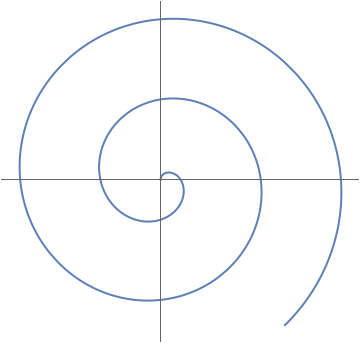
\includegraphics[keepaspectratio, scale=0.5]{fig/01.png}
      \caption{例1}
      \label{exm1}
    \end{minipage}
    \begin{minipage}[b]{0.45\linewidth}
      \centering
      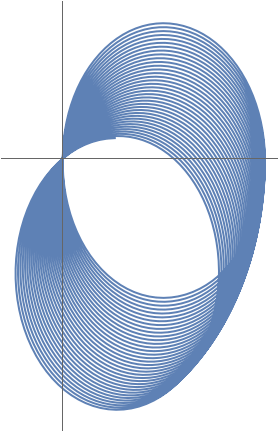
\includegraphics[keepaspectratio, scale=0.5]{fig/02.png}
      \caption{例2}
      \label{exm2}
    \end{minipage}
  \end{figure}

  微分方程式は
  \begin{equation}
    \left\{
      \begin{alignedat}{1}
        \dv[2]{x}{t}
        &=
        x
        +
        \gamma\dv{y}{t}
        \\
        \dv[2]{y}{t}
        &=
        y
        -
        \delta\dv{x}{t}
      \end{alignedat}
    \right.
  \end{equation}
  で,初期条件は$x(0)=y(0)=0,\ x'(0)=0,\ y'(0)=1$としました.$(\gamma,\delta)=(1,1)$としたのが\ref{exm1}で,$(\gamma,\delta)=(11,20)$としたのが\ref{exm2}です.

\end{enumerate}


\end{document}
